En primer lugar se tuvo que diseñar y construir un prototipo que respondiese a una serie de exigencias impuestas por el experimento. Por un lado este debía de ser capaz de albergar de manera segura  un haz de $35$ fibras centelleadoras, el cual se encontraría totalmente sumergido en una solución de agua tritiada estanca. Este prototipo debía de ser capaz de comunicar los extremos del haz con fotosensores, los cuales deben estar aislados del agua tritiada, sin que existiese ningún tipo de fisura para asegurar que no existe peligro de fuga y, por tanto, de contaminación, ni siquiera por evaporación del agua. Por otro lado, debía de sostener de forma segura el contador de fotones utilizado, en nuestro caso PMTs (marca... modelo...), para leer la señal recibida por estas fibras centelleadoras.

Con todas estas exigencias, el materíal elegido para la construcción del prototipo fueron diversos elementos de fontanería de PVC. El motivo de esta elección es su seguridad, ya que están especialmente diseñados para transportar y retener agua, su facilidad de manipulación ya que podemos realizar cortes con mucha rapidez, sencillez y eficacia además de existir muchas formas  en el mercado para diversos fines y, finalmente, su precio ya que se trata de un material bastante económico. 

En concreto se utilizó un tubo de PVC de $2~\meter$ de longitud y un diámetro interior de $15~\milli\meter$, en el cual se practicaron una serie de cortes dando lugar a un conjunto de secciones que conformarían los 2 prototipos. Para unir cada una de estas secciones y dar forma al prototipo se utilizaron codos, típicamente utilizados en fontanería de PVC, cuyas uniones serían finalmente pegadas con soldadura química. Finalmente el prototipo quedó sujeto de forma segura sobre una estructura de metacrilato y acero. Una fotografía del prototipo se muestra en la figura~\ref{prototipo}.

\begin{figure}[hbtp]
\centering
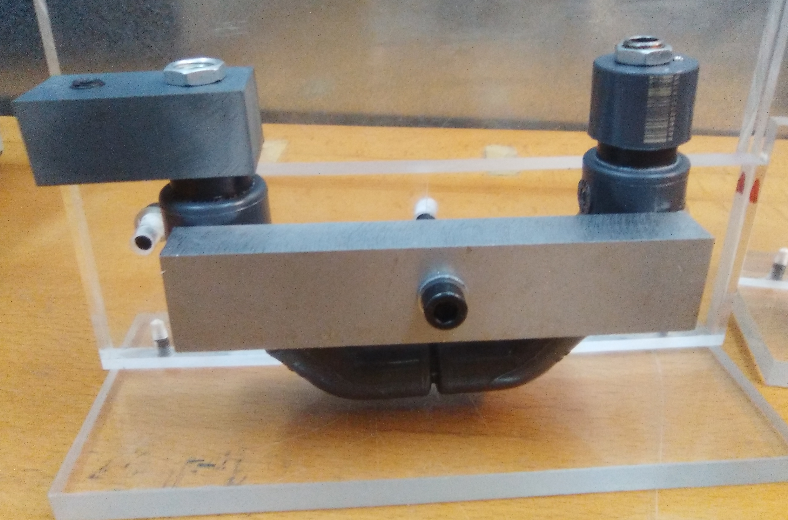
\includegraphics[scale=0.4]{Prototipo.png}
\caption{ Prototipo\label{prototipo}}
\end{figure}

Este prototipo puede contener un volumen de solución radiactiva de $39~\cm^3$, el cual se calculó y verificó con varios ensayos de llenado con agua destilada. También se verificó la ausencia de fugas del prototipomediante ensayos de 2 días. 

La forma elegida fue un prototipo en forma de U. Dado que el prototipo no se trasladará en ningún caso y, teniendo en cuenta que se verificó su estanqueidad, personalmente opino que esta es la forma más segura y que mejor se adapta a las exigencias del prototipo. Las dos oberturas superioresfueron cerradas y selladas con tapones  utilizados en fontanería de PVC y otras piezas fabricadas en el taller mecánico del IFIC. Se eligieron tapones diferentes para cada extremo. Un primer tapón circular, comercial, para tubo de PVC y un segundo tapón cuadrado, fabricado para facilitar el proceso de llenado. Este segundo tapón dispone de un orificios de $8~\milli\meter$ por el que se realizó el proceso de llenado.  All tapón circular se le practicó otro orificio de $1~\milli\meter$ para purgar el aire durante este proceso.  Estos orificios se cerraron mediante tornillos de rosca forrados de teflón, y fueron finalmente sellados con silicona. Estos tapones se muestran en la  figura~\ref{prototipo}.

Finalmente ambos extremos tienen un orificio de $10~\milli\meter$ de diámetro. Por cada uno de estos pasa un extremo del haz de fibras centelleadoras. En cada uno se dispusieron dos arandelas, roscadas al aro que formaba el extremo del haz, según la imagen~\ref{prototipo} (una arandela a cada extremo del tapón, parte interna y externa). De esta forma conseguíamos fijar perfectamente cada uno de los extremos del haz al prototipo y comunicar el extremo de las fibras al exterior del prototipo para su correspondiente lectura con los fotosensores, PMTs en nuestro caso. 
En todo momento se utilizó silicona para sellar los cierres atornillados del prototipo.

También podemos observar que se realizó el giro de $180^\circle$, correspondiente a la U, con ayuda de cuatro codos de $45^\circle$ y no con dos codos de $90^\circle$. Esto es debido a que, con giros progresivos, el haz de fibras centelleadoras estarán sometidos a una tensión inferior y, por extensión, ofrecerán una mejor propagación de la señal.

Finalmente se utilizaron dos piezas, usualmente utilizadas en fontanería de PVC para comunicar tuberías de igual o diferente diámetro para sostener los PMTs en el prototipo. Debido al hecho de haber utilizado dos tapones distintos ahora necesitaremos dos piezas diferentes. Estas pueden verse en la figura~\ref{tapones}.

\begin{figure}[hbtp]
\centering
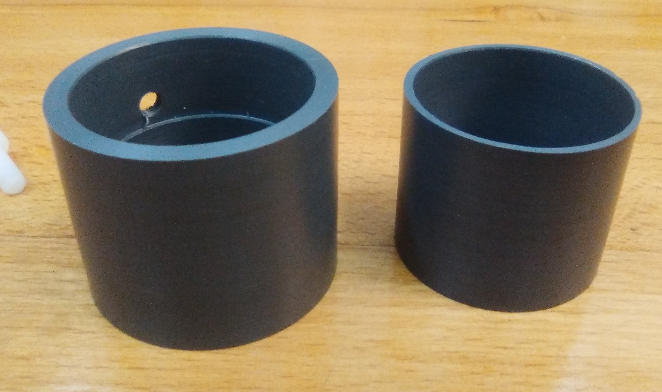
\includegraphics[scale=0.4]{Tapones.png}
\caption{Piezas de sujeción de los PMTs\label{tapones}}
\end{figure}

La primera pieza (correspondiente a la pieza derecha de esta figura), más pequeña, simplemente encajaba al tapón circular por un extremo y, por el otro, con un diámetro interior más grande para que cupiese y fijase, se disponía del PMT.

Para la segunda pieza encontramos un problema y es que no hay tuberías cuadradas, por lo que no encontramos ningún tipo de pieza como esta que ajustase a este tapón (tapón cuadrado del prototipo). En su lugar simplemente utilizamos una pieza para que encajase a la arandela que sobresalía del prototipo (utilizada para fijar el  haz de fibras) y por el otro extremo que encajase al PMT. Parauna mejor sujeción se utilizo en esta pieza un tornillo que unía esta al soporte de metacrilato. La disposición de los PMT en el prototipo y el tornillo que ayuda a la sujeción pueden observarse en la la figura~\ref\label{protipoPMT}.

\begin{figure}[htb]
\centering
{
%\subfloat[Espectro de emisión]
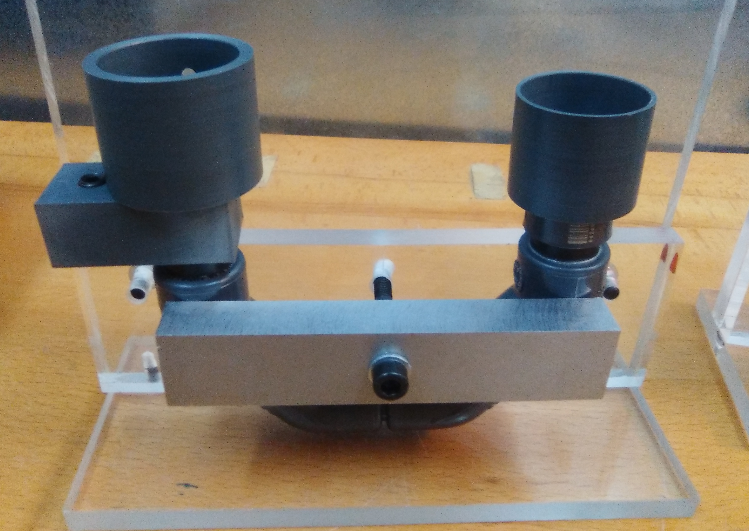
\includegraphics[scale=0.25]{Prototipodelantetapon.png} 
}
{
%\subfloat[Espectro de emisión]
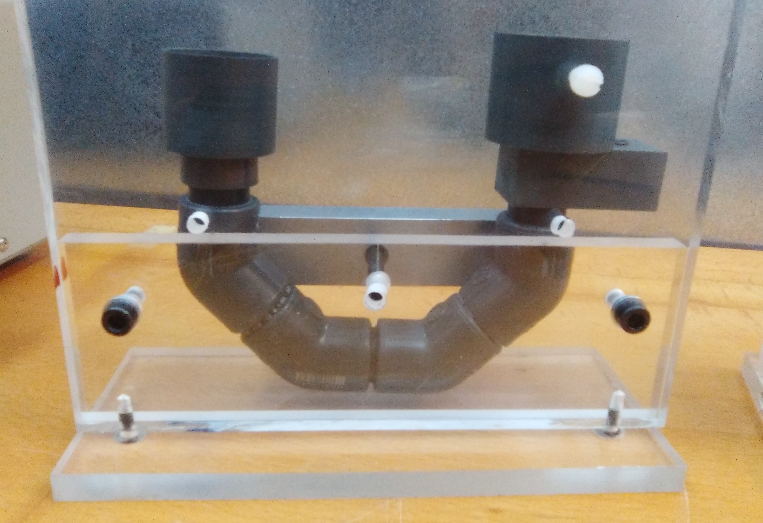
\includegraphics[scale=0.25]{PrototipoDetrastapon.png} 
}
\caption{Prototipos con piezas de sujeción de PMTs\label{protipoPMT}}
\end{figure} 


